\subsection{Hadronic Calorimeter}
Quarks and gluons produced in proton-proton collisions are not directly detected. They instead hadronize into sprays of hadrons, called jets, which we can detect, and the measured properties of the jet can then be used to infer information about the original quark or gluon. The hadronic calorimeter (HCAL) is designed to measure the energy and position of the constituent hadrons, allowing the jet to be reconstructed. This is particularly important for neutral hadrons which do not leave any hits in the inner tracker and deposit little energy in the ECAL. Furthermore, the HCAL is designed to be as hermetic as possible, covering $\abs{\eta} < 5.2$, and is deep enough such that the majority of the energy from visible particles in a collision are absorbed, except for muons which are measured in the muon system. This is crucial for a precise measurement of \ptmiss. 

The HCAL is a sampling calorimeter, with steel and brass used as the absorbing material, and plastic scintillator or quartz fibres as the active material. Hadrons shower via nuclear interactions with the detector material as they travel through the HCAL, and the light produced by this in the active material is read out via fibres. The energy of the hadrons is then inferred from the amount of light measured. The layout for one quarter of the HCAL is shown in \cref{fig:hcal}. 

\begin{figure}
  \centering
  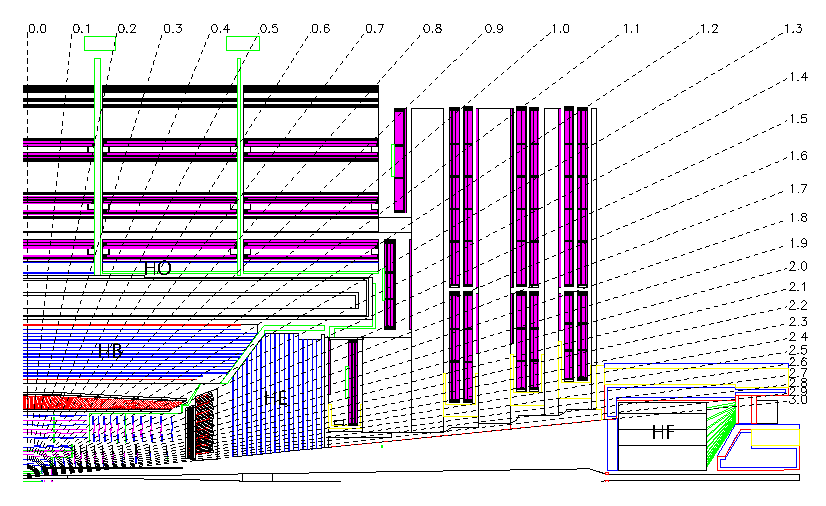
\includegraphics[width=\textwidth]{Figures/Detector/CMS/hcal.pdf}
  \caption[The CMS HCAL]{A schematic of one quarter of the HCAL in the $r$-$z$ plane. The interaction point is the lower-left corner of the diagram and the dashed lines represent constant lines of $\eta$. Figure taken from Ref.~\cite{CMS:2008xjf}.}\label{fig:hcal}
\end{figure}

The barrel (HB) extends from the ECAL to the inner coil of the CMS solenoid and covers the region $\abs{\eta} < 1.3$. Plastic scintillator is used as the active material and it is segmented into 16 $\eta$ sectors, and 72 $\phi$ sectors, leading to a granularity of $\Delta\eta \times \Delta\phi = 0.087 \times 0.087$. The thickness of the absorber corresponds to 5.82 interaction lengths ($\lambda_I$) at $\eta = 0$ and grows to 10.6 $\lambda_I$ at $\eta = 1.3$. Including the ECAL provides about 1.1 $\lambda_I$ of additional material, but this is still not enough to fully contain the hadronic showers. Therefore, an outer calorimeter (HO), with similar technology to the HB, is placed outside the solenoid and acts as a tail catcher, leading to a minimum depth of 11.8 $\lambda_I$ in the barrel region.

The hadronic calorimeter endcaps extend the coverage to $\abs{\eta} < 3$. Again, the active material is a plastic scintillator and the granularity is the same as the HB for $1.3 < \abs{\eta} < 1.6$, and reduces to $\Delta\eta \times \Delta\phi = 0.17 \times 0.17$ for $1.6 < \abs{\eta} < 3$. Including the ECAL, the total depth of the HE corresponds to about $10\lambda_I$.

The forward calorimeter (HF) extends the HCAL to its ultimate coverage of $\abs{\eta} < 5.2$. This detector will absorb 88\% of the energy produced by a proton-proton interaction and is therefore subjected to intense doses of radiation. To withstand this, quartz fibres were chosen as the active material where charged particles generate light via the Cherenkov effect. The fibres are embedded in a steel absorber and run parallel to the beam line. Since the ECAL does not cover this pseudorapidity region, the HF also designed to discriminate electromagnetic showers from hadronic ones. It does this by taking advantage of the fact that electromagnetic showers have a smaller typical depth than hadronic showers. Only half of the fibres run the full length of the HF, whereas the other half start 22~\unit{cm} from the front, therefore allowing the depth of a shower to be inferred.